\documentclass{article}
\usepackage[utf8]{inputenc}
\usepackage{listings}
\usepackage{xcolor}
\usepackage{amsmath}
\usepackage{graphicx}
\usepackage{hyperref}
\definecolor{codegreen}{rgb}{0,0.6,0}
\definecolor{codegray}{rgb}{0.5,0.5,0.5}
\definecolor{codepurple}{rgb}{0.58,0,0.82}
\definecolor{backcolour}{rgb}{0.95,0.95,0.92}
\lstdefinestyle{mystyle}{
    commentstyle=\color{codegreen},
    keywordstyle=\color{magenta},
    numberstyle=\tiny\color{codegray},
    stringstyle=\color{codepurple},
    basicstyle=\ttfamily\footnotesize,
    breakatwhitespace=false,
    breaklines=true,
    captionpos=b,
    keepspaces=true,
    showspaces=false,
    showstringspaces=false,
    showtabs=false,
    tabsize=2
}
\lstset{style=mystyle}
\title{Joint Assignment 02 Report}
\author{Anton Kudryavtsev CS-04 a.kudryavtsev@innopolis.university}
\date{\today}
\begin{document}
\maketitle
\section*{Least Square Approximation}
\paragraph*{Equation} Least Square Approximation is done using left pseudoinverse of matrix A;
\begin{equation}
    A * x = b;
\end{equation}
\begin{equation}
    A^TA * x = A^Tb;
\end{equation}
\begin{equation}
    x \approx  (A^TA)^{-1}A^Tb;
\end{equation}
\paragraph{Code.} The code to find $x$ is the following:
\begin{lstlisting}[language=c++]
int main() {
    // Specify Output Format
    std::cout.setf(std::ios::fixed, std::ios::floatfield);
    std::cout.precision(4);

    // Read Samples
    size_t m;
    std::cin >> m;
    Matrix<double> *ts = new ColumnVector<double>(m);
    Matrix<double> *b = new ColumnVector<double>(m);
    for (int i = 0; i < m; ++i) {
        double ti, bi;
        std::cin >> ti >> bi;
        ts->Put(i, 0, ti);
        b->Put(i, 0, bi);
    }
    // Read Polynomial Degree
    size_t n;
    std::cin >> n;

    // Generate Matrix A
    auto *A = new Matrix<double>(m, n+1, [ts](auto i, auto j) {
        return pow(ts->Get(i, 0), j);
    });

    // Find Model
    auto At = A->Transpose();
    auto AtA = *At * A;
    auto AtAi = AtA->Inverse();
    auto Atb = *At * b;
    auto x = *AtAi * Atb;

    // Report Steps
    std::cout << "A:\n" << A;
    std::cout << "A_T*A:\n" << AtA;
    std::cout << "(A_T*A)^-1:\n" << AtAi;
    std::cout << "A_T*b:\n" << Atb;
    std::cout << "x~:\n" << x;

    // Free Memory
    free({ts, A, b, At, AtA, AtAi, Atb, x});
    return 0;
}
\end{lstlisting}
\paragraph*{Proof.} Let us introduce function $4x^2-8x+3$ and generate samples for it with noise.
Python code:
\begin{lstlisting}[language=python]
with open("plot.dat", "w") as f:
    for i in range(1000):
        print(i, (4*i**2 -8*i +3)+(random()-0.5)*10, file=f)
\end{lstlisting}
Then, forward data from "plot.dat" file to the c++ program and get x.
We get following results:
\begin{lstlisting}
(A_T*A)^-1:
0.0865 -0.0035 0.0000
-0.0035 0.0002 0.0000
0.0000 0.0000 0.0000
A_T*b:
1274149.9855
95402091.6468
7606638251.9895
x~:
3.1682
-8.0179
4.0004
\end{lstlisting}
Plot data using \textit{gnuplot}:
\begin{lstlisting}
> set style line 1 linecolor rgb '#dd181f' linetype 1 linewidth 2
> plot "plot.dat" with points pointtype 6, [x=0:99] 4.0004 * x**2 -8.0179 * x + 3.1682 linestyle 1
\end{lstlisting}
We get following picture: \\
\graphicspath{ {./} }
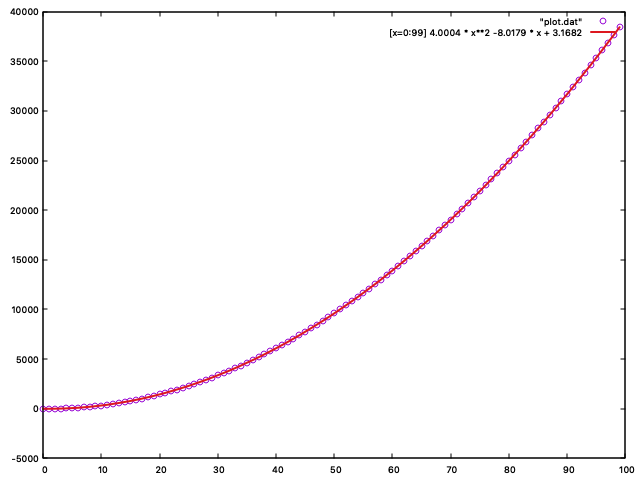
\includegraphics[scale=0.6]{plot.png}
\section*{Appendix}
Source code, "plot.dat" file and other materials could be found here: \href{https://github.com/Dartt0n/Least-Square-Approximation-Cpp}{Github}
\end{document}